In this example of acrobatic sports biomechanics, the goal was to maximize the twist rotation ($\phi$) of an 8-DoF model in a backward somersault and to illustrate \textit{bioptim}'s ability to handle quaternionic representations of rotations.
The model was composed of a 6-DoF root segment and two 1-DoF torque actuated shoulder joints.
Two different numerical descriptions of the root segment rotations were used (Euler angles and quaternions).
The objective function was as follows:

\begin{eqnarray}\label{eq:ocp_Trampo}
\mathcal{J} =  \int_0^T\underbrace{\omega_1 \dot{\phi}}_{\mathtt{MIN\_TWIST}}  + \underbrace{~\omega_2  \|\boldsymbol{\tau}\|^2}_{\mathtt{MIN\_ TORQUE}}~dt,
\end{eqnarray}
with $\omega_1 = -1$ (resulting in the maximization of the first term) and $\omega_2 = 10^{-6}$, T is the duration of the movement and $\boldsymbol{\tau}$ is the torque control vector.
The first term of the objective function (Eq.~\ref{eq:ocp_Trampo}) corresponds to maximizing the change in twist rotation and the second term is for control regularization.


The movement lasted for approximately 1 second and was discretized with 80 shooting nodes.
The optimal kinematics were different for the two types of models (Fig.~\ref{fig:snapshots_quaternion_base_twisting_somersault}) because of the presence of local minima.
However, both models take profits of a common biomechanical strategy (i.e. tilting the body to bring closer together the twist axis and the angular momentum vector) highlighting the equivalence of the two rotation representations.
Euler angles have the advantage to be easily interpretable, but they suffer from the loss of a DoF at the Gimbal lock (leading to numerical instabilities).
The use of a quaternion-based representation tackles this numerical stability issue when a joint is free to rotate on a three-dimensional range of motion.
Quaternion's integration must be handled with care~\cite{bailly2020optimal}, indeed, when representing orientations, quaternions must be unitary and thus belong to a constrained manifold (namely, the unit 3-sphere $S^3$). 
However, classical numerical integration schemes such as Runge–Kutta methods treat unit quaternions as if they were arbitrarily defined in $\mathbb{R}^4$.
This was taken care of in \textit{bioptim} by performing a normalization step after each Runge–Kutta iteration to project non-unitary quaternions onto $S^3$.



\begin{figure*}[t!]
\centering
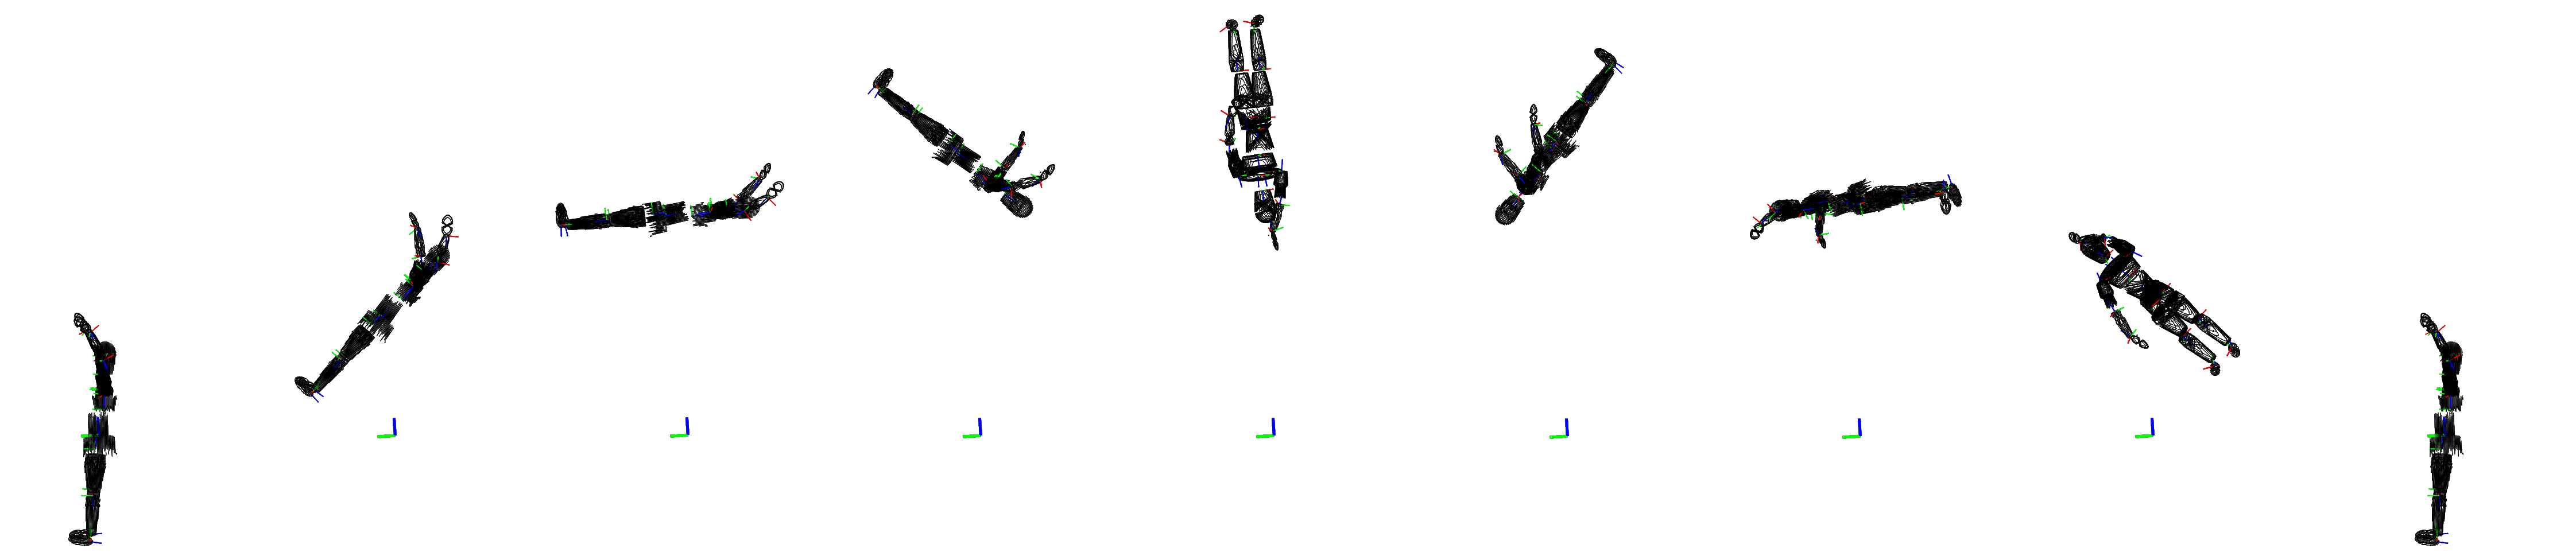
\includegraphics[width=\textwidth]{figures/Euler_Bioptim_MaxVrille_dos.png}\\
\vspace*{0.5em}
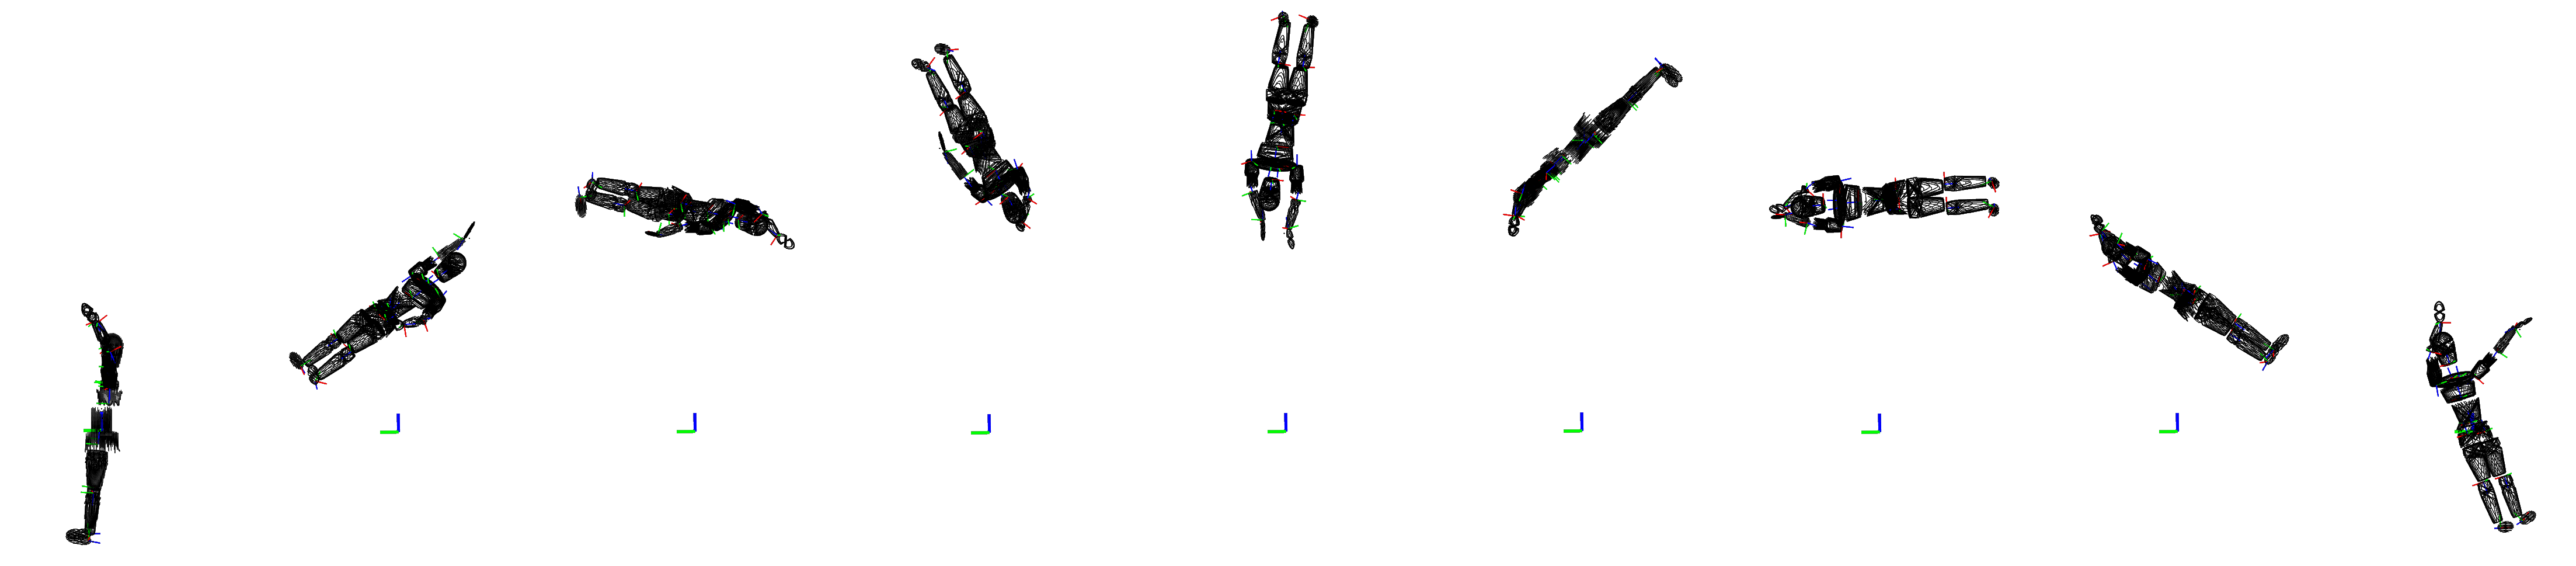
\includegraphics[width=\textwidth]{figures/Quat_Bioptim_MaxVrille_dos.png}
\caption{Snapshots of maximally twisting somersaults driven by shoulder torque actuators and a free base whose rotation is either expressed by Euler angles (top) or by quaternions (bottom).}
\label{fig:snapshots_quaternion_base_twisting_somersault}
\end{figure*}


% \begin{table}[h!]
% \caption{\small Objective terms of quaternion base maximally twisting somersault}
% \label{tab:Quaternion_base_twisting_somersault}
% \centering
% \begin{tabular}{c c c c}
% \toprule 
% & Type & Function & Weight \\ 
% \midrule
% $\#1$ & Lagrange & MINIMIZE\_TWIST & $-1e1$ \\ 
% \midrule
% $\#2$ & Lagrange & MINIMIZE\_ TORQUE & $1e-6$ \\ 
% \bottomrule
% \end{tabular}
% \end{table}













